% Source: Gerzensee "Calculus" slides 7-8, 52 (concavity and the sufficiency of
% the first-order condition; the tangent-line and tangent-plane pictures) and
% "Optimization" slides 10-18 (the concave programming problem and the role of
% concavity of objective and constraints).
% Supplementary: Fukuda (2026), Ch. 6 (convex sets, convex combinations, convex
% hull, Def. 6.1-6.2, Thm 6.1 Caratheodory, Prop. 6.3), Sec. 7.6 (topological
% structure of convex sets), Sec. 9.1 (projection onto a closed convex set),
% Ch. 10 (Def. 10.1-10.4, Prop. 10.1-10.3, Thm 10.1 First Separation, Thm 10.2
% Second Separation, Thm 10.3 Supporting Hyperplane, Thm 10.9 Farkas-Minkowski,
% Sec. 10.6.2 quasiconvexity), and Sec. 11.3 (Thm 11.3, differentiable
% concavity; Prop. 11.7, differentiable quasiconcavity).
% External references actually cited in this chapter: Aliprantis-Border
% (2006), Boyd-Vandenberghe (2004), Rockafellar (1970).

\chapter{Convexity and Separation}
\label{ch:convex}

\section{Motivation: What Convexity Buys}\label{sec:cvx-motivation}

Convexity does three things that nothing else in this volume does.

It converts local information into global information. A stationary point of a
concave function is a global maximiser (\autoref{thm:foc-concave-n}), so the
first-order conditions that \autoref{ch:calculusn} derived as necessary become
sufficient, and the search for an optimum reduces to solving equations.

It delivers uniqueness. Strict concavity of the objective on a convex feasible
set makes the solution a point rather than a set
(\autoref{prop:strict-quasi-unique}), which is what turns a demand
correspondence into a demand function and makes comparative statics well posed.

It produces prices. The separation theorems say that two disjoint convex sets can
be told apart by a linear functional --- a vector of coefficients, one per
coordinate. When the coordinates are commodities, that vector is a price system,
and the existence of supporting prices in the second welfare theorem, of state
prices under no arbitrage, and of Lagrange multipliers in
\autoref{ch:optimization} are three instances of one theorem.

\section{Convex Sets}\label{sec:cvx-sets}

\begin{definition}[Convex set]\label{def:convex-set}
	A subset $C$ of a real vector space $X$ is \dfnas{convex}{convex set} if
	\[
		\lambda x+(1-\lambda)y\in C
		\qquad\text{for all }x,y\in C\text{ and }\lambda\in[0,1] .
	\]
	Equivalently, $C$ contains the segment joining any two of its points. The empty
	set and every singleton are convex, vacuously and trivially.
\end{definition}

\begin{eg}[Convex sets in economics]\label{eg:convex-sets}
	\begin{enumerate}[(i)]
		\item The budget set $\budget(p,m)=\{x\in\R^n_+:\ip{p}{x}\leq m\}$ is convex,
		      being the intersection of the half-space $\{\ip{p}{x}\leq m\}$ with the
		      cone $\R^n_+$.
		\item The unit simplex
		      $\Delta_n=\{p\in\R^n:\sum_ip_i=1,\ p_i\geq0\}$, the set of probability
		      distributions on $n$ states, is convex and compact.
		\item An upper contour set $\{x : u(x)\geq u(x_0)\}$ is convex precisely when
		      $u$ is quasiconcave (\autoref{def:quasiconcave}); this is the formal content
		      of ``convex preferences''.
		\item A production set $Y\subseteq\R^n$ is convex when the technology admits
		      time-sharing between any two feasible plans, and convexity of $Y$ is
		      exactly what excludes increasing returns.
	\end{enumerate}
\end{eg}

\begin{proposition}[Operations preserving convexity]\label{prop:convex-operations}
	Let $C,D\subseteq\R^n$ be convex, $\lambda,\mu\in\R$, and
	$T\colon\R^n\to\R^m$ linear. Then
	\begin{enumerate}[(i)]
		\item $\bigcap_{i\in I}C_i$ is convex for any family of convex sets;
		\item $\lambda C+\mu D\eqdef\{\lambda x+\mu y : x\in C,\ y\in D\}$ is convex;
		\item $T(C)\subseteq\R^m$ and $T^{-1}(E)\subseteq\R^n$ are convex, the latter
		      for any convex $E\subseteq\R^m$;
		\item $\Int C$ and $\closure C$ are convex.
	\end{enumerate}
\end{proposition}

\begin{proof}
	(i) If $x,y\in\bigcap_iC_i$ then the segment lies in each $C_i$.

	(ii) Let $z_k=\lambda x_k+\mu y_k$ for $k=1,2$ and $\theta\in[0,1]$. Then
	$\theta z_1+(1-\theta)z_2=\lambda\bigl(\theta x_1+(1-\theta)x_2\bigr)
		+\mu\bigl(\theta y_1+(1-\theta)y_2\bigr)$, and both brackets lie in the
	respective sets.

	(iii) Immediate from linearity of $T$, which commutes with convex combinations.

	(iv) For the closure: let $x,y\in\closure C$ and take
	$(x_k),(y_k)\subseteq C$ with $x_k\to x$, $y_k\to y$
	(\autoref{thm:closed-sequential}). Then
	$\lambda x_k+(1-\lambda)y_k\in C$ converges to $\lambda x+(1-\lambda)y$, which
	is therefore in $\closure C$. For the interior: let $x,y\in\Int C$ with
	$\ball{\varepsilon}{x},\ball{\varepsilon}{y}\subseteq C$ and set
	$z=\lambda x+(1-\lambda)y$. For $\norm{u}<\varepsilon$,
	$z+u=\lambda(x+u)+(1-\lambda)(y+u)\in C$, so
	$\ball{\varepsilon}{z}\subseteq C$.
\end{proof}

This is Proposition~6.3 and the results of Section~7.6 of
\textcite{fukuda2026notes}. Part (i) is the one used most often: a feasible set
described by a list of convex constraints is convex, however long the list, and
part (ii) is what makes the aggregate of convex production sets convex.

\begin{definition}[Convex combination and convex hull]\label{def:convex-hull}
	A point $a\in\R^n$ is a \dfn{convex combination} of $x_1,\dots,x_k$ if
	$a=\sum_{i=1}^k\lambda_ix_i$ with $\lambda_i\geq0$ and
	$\sum_{i=1}^k\lambda_i=1$. The \dfn{convex hull} $\conv A$ of $A\subseteq\R^n$
	is the set of all convex combinations of finitely many points of $A$;
	equivalently, by \autoref{prop:convex-operations}(i), the intersection of all
	convex sets containing $A$, hence the smallest such set.
	\nidx{conv}{$\conv A$, convex hull}
\end{definition}

\begin{theorem}[Carath\'eodory]\label{thm:caratheodory}
	Let $A\subseteq\R^n$. Every point of $\conv A$ is a convex combination of at
	most $n+1$ points of $A$.
\end{theorem}

\begin{proof}
	Let $x=\sum_{i=1}^{k}\lambda_ix_i$ with $x_i\in A$, $\lambda_i>0$,
	$\sum_i\lambda_i=1$, and suppose $k\geq n+2$. The $k-1\geq n+1$ vectors
	$x_2-x_1,\dots,x_k-x_1$ lie in $\R^n$ and are therefore linearly dependent:
	there are $\mu_2,\dots,\mu_k$, not all zero, with
	$\sum_{i=2}^{k}\mu_i(x_i-x_1)=0$. Setting $\mu_1\eqdef-\sum_{i\geq2}\mu_i$
	gives $\sum_{i=1}^k\mu_ix_i=0$ and $\sum_{i=1}^k\mu_i=0$, with some
	$\mu_i>0$ because they sum to zero and are not all zero.

	For $t\geq0$ the coefficients $\lambda_i-t\mu_i$ still sum to $1$ and still
	represent $x$. Let
	$t^\ast\eqdef\min\{\lambda_i/\mu_i : \mu_i>0\}$, attained at some index $j$. Then
	$\lambda_i-t^\ast\mu_i\geq0$ for every $i$ and equals $0$ at $i=j$, so $x$ is a
	convex combination of the remaining $k-1$ points. Iterate until $k\leq n+1$.
\end{proof}

This is Theorem~6.1 of \textcite[p.~190]{fukuda2026notes}. The bound $n+1$ is
sharp --- a point in the interior of a simplex in $\R^n$ needs all $n+1$
vertices --- and the theorem is the reason that finitely many agents suffice to
generate any aggregate consumption bundle in an $n$-commodity economy.

\begin{lemma}[Nearest point in a closed convex set]\label{lem:nearest-point}
	Let $\emptyset\neq D\subseteq\R^n$ be closed and convex and let $x\in\R^n$.
	Then there is exactly one $P_Dx\in D$ with
	\[
		\norm{x-P_Dx}=\dist(x,D)\eqdef\inf_{y\in D}\norm{x-y},
	\]
	and $P_Dx$ is characterised by the variational inequality
	\begin{equation}\label{eq:variational-inequality}
		\ip{x-P_Dx}{y-P_Dx}\leq0\qquad\text{for all }y\in D .
	\end{equation}
\end{lemma}

\begin{proof}
	\emph{Existence.} Fix $y_0\in D$ and set $R\eqdef\norm{x-y_0}$. The set
	$D\cap\closure{\ball{R}{x}}$ is non-empty, closed and bounded, hence compact by
	\autoref{thm:heine-borel}, and the continuous function $y\mapsto\norm{x-y}$
	attains its minimum there by \autoref{cor:weierstrass-continuous}. That minimum
	is the infimum over all of $D$, since points outside the ball are further away
	than $y_0$.

	\emph{Uniqueness.} Let $d\eqdef\dist(x,D)$ and suppose
	$\norm{x-y_1}=\norm{x-y_2}=d$ with $y_1\neq y_2$. The midpoint
	$\bar y=\tfrac12(y_1+y_2)$ lies in $D$ by convexity, and the parallelogram law
	(\autoref{rem:parallelogram}) gives
	\[
		\norm{x-\bar y}^2=\tfrac12\norm{x-y_1}^2+\tfrac12\norm{x-y_2}^2
		-\tfrac14\norm{y_1-y_2}^2=d^2-\tfrac14\norm{y_1-y_2}^2<d^2,
	\]
	contradicting minimality of $d$.

	\emph{Characterisation.} Let $z\eqdef P_Dx$, $y\in D$ and $t\in(0,1]$. Then
	$z+t(y-z)\in D$, so
	\[
		\norm{x-z}^2\leq\norm{x-z-t(y-z)}^2
		=\norm{x-z}^2-2t\ip{x-z}{y-z}+t^2\norm{y-z}^2 .
	\]
	Cancelling, dividing by $t>0$ and letting $t\downarrow0$ gives
	\eqref{eq:variational-inequality}. Conversely, if $z\in D$ satisfies
	\eqref{eq:variational-inequality}, then for any $y\in D$,
	\[
		\norm{x-y}^2=\norm{x-z}^2-2\ip{x-z}{y-z}+\norm{y-z}^2\geq\norm{x-z}^2 ,
	\]
	so $z$ is the minimiser.
\end{proof}

This is the finite-dimensional case of Theorem~9.1 of
\textcite[p.~295]{fukuda2026notes}. The Hilbert-space version, in which
compactness is unavailable and completeness does the work instead, is
\autoref{thm:projection-convex}; the uniqueness and variational arguments above
carry over verbatim, and only the existence argument changes.

\section{Convex and Concave Functions}\label{sec:cvx-functions}

\begin{definition}[Convexity and concavity]\label{def:convex-function}
	Let $C\subseteq\R^n$ be convex. A function $f\colon C\to\R$ is
	\dfnas{convex}{convex function!on $\R^n$} if
	\[
		f\bigl(\lambda x+(1-\lambda)y\bigr)\leq\lambda f(x)+(1-\lambda)f(y)
		\qquad\text{for all }x,y\in C,\ \lambda\in[0,1],
	\]
	\dfn{strictly convex} if the inequality is strict for $x\neq y$ and
	$\lambda\in(0,1)$, and \dfnas{concave}{concave function!on $\R^n$}
	(respectively strictly concave) if $-f$ is convex (respectively strictly
	convex).
\end{definition}

\begin{proposition}[Epigraph and Jensen]\label{prop:convex-epigraph}
	Let $C\subseteq\R^n$ be convex and $f\colon C\to\R$.
	\begin{enumerate}[(i)]
		\item $f$ is convex if and only if $\epi f=\{(x,z)\in C\times\R : f(x)\leq z\}$
		      is a convex subset of $\R^{n+1}$.
		\item If $f$ is convex, then for all $x_1,\dots,x_k\in C$ and weights
		      $\lambda_i\geq0$ with $\sum_i\lambda_i=1$,
		      \begin{equation}\label{eq:jensen-finite}
			      f\Bigl(\sum_{i=1}^{k}\lambda_ix_i\Bigr)\leq\sum_{i=1}^{k}\lambda_if(x_i).
		      \end{equation}
	\end{enumerate}
\end{proposition}

\begin{proof}
	(i) Suppose $f$ convex and $(x_1,z_1),(x_2,z_2)\in\epi f$. For
	$\lambda\in[0,1]$,
	$f(\lambda x_1+(1-\lambda)x_2)\leq\lambda f(x_1)+(1-\lambda)f(x_2)
		\leq\lambda z_1+(1-\lambda)z_2$, so the convex combination is in $\epi f$.
	Conversely, apply convexity of $\epi f$ to the points $(x_i,f(x_i))$.

	(ii) Induction on $k$. The case $k=2$ is the definition. For the step, if
	$\lambda_k<1$ write $\sum_{i\leq k}\lambda_ix_i
		=(1-\lambda_k)\sum_{i<k}\frac{\lambda_i}{1-\lambda_k}x_i+\lambda_kx_k$, apply
	the definition, and then the inductive hypothesis to the inner combination,
	whose weights sum to $1$.
\end{proof}

Combining \autoref{prop:convex-epigraph}(i) with \autoref{prop:epigraph} gives
the identification announced in \autoref{ch:continuity}: $f$ is convex and lower
semicontinuous exactly when $\epi f$ is a closed convex set. Inequality
\eqref{eq:jensen-finite} is Jensen's inequality for a finitely supported
distribution; the general version, for an arbitrary distribution and for
conditional expectations, is \autoref{prop:conditional-jensen}.

\begin{proposition}[Operations]\label{prop:convex-function-operations}
	Let $C\subseteq\R^n$ be convex.
	\begin{enumerate}[(i)]
		\item If $f,g$ are convex and $\alpha,\beta\geq0$, then $\alpha f+\beta g$ is
		      convex.
		\item If $(f_i)_{i\in I}$ are convex and $f=\sup_{i\in I}f_i$ is finite on
		      $C$, then $f$ is convex. The corresponding statement for infima of concave
		      functions holds; suprema of concave functions need not be concave.
		\item If $f$ is convex and $\varphi\colon\R\to\R$ is convex and
		      non-decreasing, then $\varphi\circ f$ is convex.
		\item If $T$ is affine, $f\circ T$ is convex whenever $f$ is.
	\end{enumerate}
\end{proposition}

\begin{proof}
	(i) and (iv) are immediate from the definition. (ii) is
	$\epi\bigl(\sup_if_i\bigr)=\bigcap_i\epi f_i$ together with
	\autoref{prop:convex-operations}(i) and \autoref{prop:convex-epigraph}(i).
	(iii): $\varphi(f(\lambda x+(1-\lambda)y))\leq\varphi(\lambda
		f(x)+(1-\lambda)f(y))\leq\lambda\varphi(f(x))+(1-\lambda)\varphi(f(y))$, the
	first step by monotonicity of $\varphi$ and convexity of $f$, the second by
	convexity of $\varphi$. Monotonicity cannot be dropped: $\varphi(t)=t^2$ is
	convex, $f(x)=-x$ is convex, and $\varphi\circ f=x^2$ happens to be convex, but
	with $f(x)=\abs{x}-1$ and $\varphi(t)=-t$ the composition is concave.
\end{proof}

Part (ii) is the source of the profit function's convexity in prices, as
\autoref{ex:cont-3} noted: $\pi(p)=\sup_{y\in Y}\ip{p}{y}$ is a supremum of
linear, hence convex, functions of $p$, and the conclusion holds for any
production set whatsoever, convex or not.

\begin{proposition}[Continuity]\label{prop:convex-continuous}
	A convex function on an open convex set $C\subseteq\R^n$ is continuous on $C$,
	and Lipschitz on every compact subset of $C$.
\end{proposition}

The proof is a standard argument bounding a convex function on a simplex by its
values at the vertices; see \textcite[Thm.~10.4]{rockafellar1970convex}. The
openness hypothesis is essential: $f(x)=0$ on $[0,1)$ and $f(1)=1$ is convex on
$[0,1]$ and discontinuous at the endpoint. In economics this is why boundary
behaviour of convex cost or value functions requires separate attention even when
the interior behaviour is smooth.

\begin{theorem}[Differentiable characterisation]\label{thm:concave-gradient}
	Let $C\subseteq\R^n$ be open and convex and $f\colon C\to\R$ differentiable.
	The following are equivalent.
	\begin{enumerate}[(i)]
		\item $f$ is concave on $C$.
		\item $f(x)\leq f(x_0)+\ip{\nabla f(x_0)}{x-x_0}$ for all $x,x_0\in C$.
		\item $\ip{\nabla f(x)-\nabla f(x_0)}{x-x_0}\leq0$ for all $x,x_0\in C$, that
		      is, $\nabla f$ is monotone decreasing.
	\end{enumerate}
	If $f$ is twice differentiable, each is equivalent to $\Hess f\preceq0$ on $C$
	(\autoref{thm:hessian-convexity}). The convex case is obtained by reversing
	every inequality.
\end{theorem}

\begin{proof}
	Fix $x,x_0\in C$ and set $\varphi(t)\eqdef f\bigl(x_0+t(x-x_0)\bigr)$ on an
	open interval containing $[0,1]$. By \autoref{thm:chain-rule},
	$\varphi'(t)=\ip{\nabla f(x_0+t(x-x_0))}{x-x_0}$.

	$f$ is concave on $C$ if and only if every such $\varphi$ is concave, since the
	defining inequality for $f$ at the pair $(x,x_0)$ is the inequality for
	$\varphi$ at the pair $(1,0)$ and conversely. By
	\autoref{thm:concave-tangent}, $\varphi$ concave is equivalent to
	$\varphi(1)\leq\varphi(0)+\varphi'(0)$, which is (ii), and to $\varphi'$
	non-increasing, which evaluated at $t=0$ and $t=1$ is (iii).
\end{proof}

This is Theorem~11.3 of \textcite[p.~388]{fukuda2026notes}. Statement (ii) is
the tangent-plane picture of \autocite[slides 8, 52]{fukuda2026calculus}: a
concave function lies below each of its tangent hyperplanes, which is why a
horizontal tangent certifies a global maximum.

\subsection{Quasiconcavity}

\begin{definition}[Quasiconcavity]\label{def:quasiconcave}
	Let $C\subseteq\R^n$ be convex. A function $f\colon C\to\R$ is
	\dfnas{quasiconcave}{quasiconcave function} if every upper contour set
	$\{x\in C : f(x)\geq\alpha\}$ is convex, equivalently if
	\[
		f\bigl(\lambda x+(1-\lambda)y\bigr)\geq\min\{f(x),f(y)\}
		\qquad\text{for all }x,y\in C,\ \lambda\in[0,1] .
	\]
	It is \dfn{strictly quasiconcave} if the inequality is strict whenever
	$x\neq y$ and $\lambda\in(0,1)$. Quasiconvexity is the same with lower contour
	sets and $\max$.
\end{definition}

\begin{proposition}\label{prop:concave-implies-quasiconcave}
	Every concave function is quasiconcave, and quasiconcavity is preserved by
	strictly increasing transformations of the values, whereas concavity is not.
\end{proposition}

\begin{proof}
	If $f$ is concave then
	$f(\lambda x+(1-\lambda)y)\geq\lambda f(x)+(1-\lambda)f(y)
		\geq\min\{f(x),f(y)\}$. For the second claim, let $\psi$ be strictly
	increasing. The upper contour sets of $\psi\circ f$ are upper contour sets of
	$f$, since $\psi(f(x))\geq\alpha$ if and only if
	$f(x)\geq\psi^{-1}(\alpha)$ on the range; convexity of the latter is
	quasiconcavity of $f$. That concavity is not preserved is shown by
	$f(x)=x$ on $\R$, concave, and $\psi(t)=t^3$, giving the non-concave $x^3$.
\end{proof}

The asymmetry in \autoref{prop:concave-implies-quasiconcave} is the reason
quasiconcavity, not concavity, is the right hypothesis on a utility function.
Utility is an ordinal representation of a preference relation, unique only up to
strictly increasing transformation, and convexity of preferences --- convexity of
the sets $\{y : y\succsim x\}$ --- is exactly quasiconcavity of every
representation. Concavity, by contrast, is a property of a particular
representation and has no preference-level meaning.

\begin{proposition}[Uniqueness of the maximiser]\label{prop:strict-quasi-unique}
	Let $C\subseteq\R^n$ be convex and $f\colon C\to\R$ strictly quasiconcave. Then
	$f$ has at most one maximiser on $C$. If in addition $C$ is compact and
	non-empty and $f$ is upper semicontinuous, the maximiser exists and is unique.
\end{proposition}

\begin{proof}
	Suppose $x\neq y$ both maximise $f$ on $C$, with common value $M$. Then
	$\tfrac12x+\tfrac12y\in C$ and strict quasiconcavity gives
	$f\bigl(\tfrac12x+\tfrac12y\bigr)>\min\{f(x),f(y)\}=M$, contradicting
	maximality. Existence is \autoref{thm:weierstrass}(ii).
\end{proof}

\begin{proposition}[Differentiable quasiconcavity]\label{prop:quasiconcave-gradient}
	Let $C\subseteq\R^n$ be open and convex and $f\colon C\to\R$ differentiable.
	Then $f$ is quasiconcave if and only if
	\[
		f(x)\geq f(x_0)\quad\Longrightarrow\quad\ip{\nabla f(x_0)}{x-x_0}\geq0
		\qquad\text{for all }x,x_0\in C .
	\]
\end{proposition}

This is Proposition~11.7 of \textcite[p.~396]{fukuda2026notes}. The condition
says that moving from $x_0$ towards any weakly preferred point does not initially
decrease $f$; geometrically the gradient at $x_0$ supports the upper contour set
at $x_0$. It is weaker than \autoref{thm:concave-gradient}(ii), which bounds $f$
globally, and correspondingly it does \emph{not} make a stationary point a global
maximiser: $f(x)=x^3$ is quasiconcave on $\R$ with $f'(0)=0$ and $0$ is not a
maximiser. Under quasiconcavity the first-order condition remains only necessary,
which is why \autoref{ch:optimization} states its sufficiency results under
concavity and treats quasiconcavity separately.

\section{Hyperplanes and Separation}\label{sec:cvx-separation}

\begin{definition}[Hyperplane and half-spaces]\label{def:hyperplane}
	A \dfn{hyperplane} in $\R^n$ is a set of the form
	\[
		H_{a,\alpha}\eqdef\{x\in\R^n : \ip{a}{x}=\alpha\},
		\qquad a\in\R^n\setminus\{0\},\ \alpha\in\R,
	\]
	equivalently an affine subspace of dimension $n-1$. It determines the two
	closed \dfnas{half-spaces}{half-space} $\{\ip{a}{x}\geq\alpha\}$ and
	$\{\ip{a}{x}\leq\alpha\}$. The hyperplane \dfnas{separates}{separating
		hyperplane} $A$ and $B$ if
	\[
		\ip{a}{x}\geq\alpha\geq\ip{a}{y}\qquad\text{for all }x\in A,\ y\in B,
	\]
	and \dfnas{strictly separates}{strict separation} them if both inequalities can
	be taken strict with a gap, that is if $\sup_{y\in B}\ip{a}{y}<\alpha<
		\inf_{x\in A}\ip{a}{x}$.
\end{definition}

That every hyperplane has the stated form is Proposition~10.1 of
\textcite[p.~334]{fukuda2026notes}, and it is \autoref{thm:riesz-rn} in
disguise: an affine subspace of codimension $1$ is a level set of a non-zero
linear functional, and every such functional is an inner product with a fixed
vector.

\begin{lemma}[Separating a point from a closed convex set]\label{lem:point-separation}
	Let $D\subseteq\R^n$ be non-empty, closed and convex and let $x\notin D$. Then
	there are $a\in\R^n\setminus\{0\}$ and $\alpha\in\R$ with
	\[
		\ip{a}{x}>\alpha>\ip{a}{y}\qquad\text{for all }y\in D .
	\]
\end{lemma}

\begin{proof}
	Let $z\eqdef P_Dx$ from \autoref{lem:nearest-point} and put
	$a\eqdef x-z\neq0$, since $x\notin D$ and $z\in D$. By
	\eqref{eq:variational-inequality}, $\ip{a}{y-z}\leq0$, that is
	$\ip{a}{y}\leq\ip{a}{z}$ for every $y\in D$. Also
	\[
		\ip{a}{x}-\ip{a}{z}=\ip{a}{x-z}=\norm{a}^2>0 .
	\]
	Any $\alpha$ strictly between $\ip{a}{z}$ and $\ip{a}{x}$ --- for instance
	$\alpha=\ip{a}{z}+\tfrac12\norm{a}^2$ --- works.
\end{proof}

\begin{theorem}[Strict separation]\label{thm:separation-2}
	Let $C,D\subseteq\R^n$ be non-empty, convex and disjoint, with $C$ compact and
	$D$ closed. Then there is a hyperplane strictly separating them.
\end{theorem}

\begin{proof}
	The set $E\eqdef C+(-D)=\{x-y : x\in C,\ y\in D\}$ is convex by
	\autoref{prop:convex-operations}(ii), and $0\notin E$ because $C\cap D=\emptyset$.
	It is closed: if $x_k-y_k\to w$ with $x_k\in C$ and $y_k\in D$, compactness of
	$C$ gives a subsequence $x_{k_j}\to x\in C$, whence
	$y_{k_j}=x_{k_j}-(x_{k_j}-y_{k_j})\to x-w$, which lies in $D$ because $D$ is
	closed; so $w=x-(x-w)\in E$.

	Apply \autoref{lem:point-separation} to the closed convex set $E$ and the point
	$0\notin E$: there are $b\neq0$ and $\alpha_0$ with
	$0=\ip{b}{0}>\alpha_0>\ip{b}{w}$ for every $w\in E$, that is
	\[
		\ip{b}{x}-\ip{b}{y}<\alpha_0<0
		\qquad\text{for all }x\in C,\ y\in D .
	\]
	Taking the supremum over $x\in C$ and the infimum over $y\in D$,
	\[
		\sup_{x\in C}\ip{b}{x}\;\leq\;\inf_{y\in D}\ip{b}{y}+\alpha_0
		\;<\;\inf_{y\in D}\ip{b}{y},
	\]
	so the two quantities are separated by the strictly positive gap
	$\abs{\alpha_0}$. Setting $a\eqdef-b$ and taking $\alpha$ to be $-1$ times the
	midpoint of the two bounds gives
	$\inf_{x\in C}\ip{a}{x}>\alpha>\sup_{y\in D}\ip{a}{y}$, which is strict
	separation in the orientation of \autoref{def:hyperplane}.
\end{proof}

\begin{theorem}[Supporting hyperplane]\label{thm:supporting-hyperplane}
	Let $C\subseteq\R^n$ be non-empty and convex, not necessarily closed, and let
	$x_0\in\partial C$. Then there is $a\in\R^n\setminus\{0\}$ with
	\[
		\ip{a}{x}\leq\ip{a}{x_0}\qquad\text{for all }x\in C .
	\]
\end{theorem}

\begin{proof}
	Since $x_0\in\partial C=\closure C\setminus\Int C$, there is a sequence
	$(x_k)\subseteq\comp{\bigl(\closure C\bigr)}$ with $x_k\to x_0$. For each $k$,
	\autoref{lem:point-separation} applied to the closed convex set $\closure C$
	and the point $x_k$ supplies $a_k\neq0$ with
	$\ip{a_k}{x}<\ip{a_k}{x_k}$ for all $x\in\closure C$; normalising,
	$\norm{a_k}=1$. The unit sphere in $\R^n$ is compact by
	\autoref{thm:heine-borel}, so a subsequence converges, $a_{k_j}\to a$ with
	$\norm{a}=1$, hence $a\neq0$. For fixed $x\in C$,
	$\ip{a_{k_j}}{x}<\ip{a_{k_j}}{x_{k_j}}$ for every $j$; letting $j\to\infty$ and
	using continuity of the inner product gives $\ip{a}{x}\leq\ip{a}{x_0}$.
\end{proof}

This is Theorem~10.3 of \textcite[p.~343]{fukuda2026notes}. The proof is an
instance of a recurring pattern: obtain the result at nearby points where a
stronger theorem applies, normalise, and extract a convergent subsequence by
compactness of the sphere --- a step available only in finite dimensions, which
is why the infinite-dimensional supporting hyperplane theorem requires
non-empty interior or a different argument \autocite[Ch.~7]{aliprantis2006infinite}.
\autoref{fig:separation} contrasts the two conclusions: strict separation puts a
gap on each side of the hyperplane, support allows the hyperplane to touch.

\begin{figure}[htbp]
	\centering
	% Figures/separation.tex
% Illustrates Definition \ref{def:hyperplane}, Theorem \ref{thm:separation-2}
% (strict separation) and Theorem \ref{thm:supporting-hyperplane} of Chapter
% \ref{ch:convexity}.
% Source: Fukuda (2026), Supplementary Ch. 10, Sec. 10.2 (pp. 334-345).
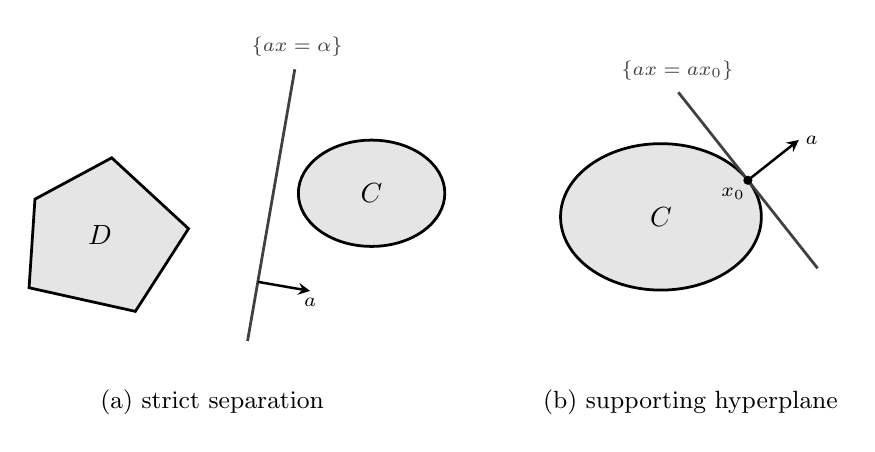
\begin{tikzpicture}[
		scale=1.5,
		>=stealth,
		setline/.style={line width=1pt,black,fill=black!10},
		hyper/.style={line width=1pt,black!75},
		normalarrow/.style={->,line width=0.9pt,black},
		panel/.style={font=\small},
	]

	% ---------- panel A: strict separation ----------
	\begin{scope}
		\filldraw[setline] (0.15,0.35) -- (1.05,0.15) -- (1.50,0.85) --
		(0.85,1.45) -- (0.20,1.10) -- cycle;
		\node at (0.75,0.80) {$D$};
		\filldraw[setline] (3.05,1.15) ellipse [x radius=0.62, y radius=0.45];
		\node at (3.05,1.15) {$C$};
		\draw[hyper] (2.00,-0.10) -- (2.40,2.20);
		\node[hyper,anchor=south,font=\scriptsize] at (2.42,2.22)
		{$\{\ip{a}{x}=\alpha\}$};
		\draw[normalarrow] (2.087,0.40) -- ++(0.443,-0.077)
		node[below,font=\scriptsize,inner sep=2pt] {$a$};
		\node[panel] at (1.70,-0.62) {(a) strict separation};
	\end{scope}

	% ---------- panel B: supporting hyperplane ----------
	\begin{scope}[shift={(4.30,0)}]
		\filldraw[setline] (1.20,0.95) ellipse [x radius=0.85, y radius=0.62];
		\node at (1.20,0.95) {$C$};
		\draw[hyper] (2.526,0.515) -- (1.347,2.005);
		\node[hyper,anchor=south,font=\scriptsize] at (1.34,2.02)
		{$\{\ip{a}{x}=\ip{a}{x_0}\}$};
		\fill (1.936,1.260) circle (1.1pt);
		\node[anchor=north east,font=\scriptsize,inner sep=1.5pt]
		at (1.95,1.235) {$x_0$};
		\draw[normalarrow] (1.936,1.260) -- ++(0.431,0.341)
		node[right,font=\scriptsize,inner sep=2pt] {$a$};
		\node[panel] at (1.45,-0.62) {(b) supporting hyperplane};
	\end{scope}

\end{tikzpicture}

	\caption[Separation and support]{The two geometries. In (a) the sets are
		disjoint, one of them compact, and the hyperplane passes strictly between
		them with a gap on each side, so
		$\sup_{y\in D}\ip{a}{y}<\alpha<\inf_{x\in C}\ip{a}{x}$
		(\autoref{thm:separation-2}). In (b) the hyperplane touches $C$ at a
		boundary point and leaves the whole set in one closed half-space, so
		$\ip{a}{x}\leq\ip{a}{x_0}$ for every $x\in C$
		(\autoref{thm:supporting-hyperplane}). In both panels $a$ points into the
		half-space on which $\ip{a}{\cdot}$ is larger, which is toward $C$ in (a)
		and away from $C$ in (b): the two statements orient the normal
		oppositely, and replacing $a$ by $-a$ converts either into the other.}
	\label{fig:separation}
\end{figure}

\begin{theorem}[Separation]\label{thm:separation-1}
	Let $C,D\subseteq\R^n$ be non-empty, convex and disjoint. Then there is a
	hyperplane separating them; moreover the separating inequality is strict on
	$\Int C$ whenever $\Int C\neq\emptyset$.
\end{theorem}

\begin{proof}
	As above, $E=C+(-D)$ is convex with $0\notin E$. If $0\notin\closure E$, apply
	\autoref{lem:point-separation} to $\closure E$, which is convex by
	\autoref{prop:convex-operations}(iv). If $0\in\closure E$, then $0\in\partial E$,
	since $0\notin E$ excludes $0\in\Int E$, and
	\autoref{thm:supporting-hyperplane} applied to $E$ at its boundary point $0$
	supplies $a\neq0$ with $\ip{a}{w}\leq\ip{a}{0}=0$ for all $w\in E$. In both
	cases $\ip{a}{x}\leq\ip{a}{y}$ for all $x\in C$ and $y\in D$, so with
	$\alpha\eqdef\sup_{x\in C}\ip{a}{x}$, which is finite and at most
	$\inf_{y\in D}\ip{a}{y}$,
	\[
		\ip{a}{x}\leq\alpha\leq\ip{a}{y}\qquad\text{for all }x\in C,\ y\in D,
	\]
	which is separation in the sense of \autoref{def:hyperplane}, with the roles of
	the two sets interchanged.

	Strictness on $\Int C$: suppose $\ip{a}{x_0}=\alpha$ for some
	$x_0\in\Int C$. Then $x_0+\varepsilon a\in C$ for small $\varepsilon>0$, and
	$\ip{a}{x_0+\varepsilon a}=\alpha+\varepsilon\norm{a}^2>\alpha$, contradicting
	the inequality just established.
\end{proof}

These are Theorems~10.1 and~10.2 of \textcite[pp.~337, 339]{fukuda2026notes},
and \textcite[Sec.~2.5, p.~46]{boyd2004convex} states the same pair in the form
used by the optimisation literature;
the compactness hypothesis in \autoref{thm:separation-2} is what upgrades
separation to strict separation and cannot be dropped. The standard witness is
$C=\{(x_1,x_2) : x_2\geq e^{x_1}\}$ and $D=\{(x_1,0) : x_1\in\R\}$: both are
closed and convex and disjoint, the separating hyperplane $x_2=0$ is unique, and
no strict separation exists because $\dist(C,D)=0$.

\section{The Farkas--Minkowski Theorem}\label{sec:cvx-farkas}

\begin{theorem}[Farkas--Minkowski]\label{thm:farkas}
	Let $f,g_1,\dots,g_m\colon\R^n\to\R$ be concave, and let
	$q\in\{0,1,\dots,m\}$ be such that $g_i$ is affine for
	$i\in\{q+1,\dots,m\}$. Assume the system
	\begin{equation}\label{eq:slater}
		g_i(x)>0\ \ (i\leq q),\qquad g_i(x)\geq0\ \ (i>q)
	\end{equation}
	has a solution. Then the system
	\begin{equation}\label{eq:farkas-system}
		f(x)>0\quad\text{and}\quad g_i(x)\geq0\ \ (i=1,\dots,m)
	\end{equation}
	has no solution in $\R^n$ if and only if there exists
	$y=(y_1,\dots,y_m)\in\R^m_+$ such that
	\[
		\sup_{x\in\R^n}\ \Bigl\{f(x)+\sum_{i=1}^{m}y_ig_i(x)\Bigr\}\leq0 .
	\]
\end{theorem}

This is Theorem~10.9 of \textcite[p.~353]{fukuda2026notes}, proved there from
\autoref{thm:separation-1} applied to the convex set
$\bigl\{(f(x),g_1(x),\dots,g_m(x))+\R^{m+1}_{--} : x\in\R^n\bigr\}$ and the
non-negative orthant. The proof is not reproduced here; it is a page of careful
bookkeeping with no additional economic content, and the statement is used only
through \autoref{ch:optimization}.

The theorem is the mechanism by which multipliers appear. Read
\eqref{eq:farkas-system} as ``no feasible point strictly improves on the
candidate'': $f$ is the improvement in the objective and the $g_i$ are the
constraints. The conclusion produces non-negative numbers $y_i$ --- the
multipliers --- such that the aggregate $f+\sum_iy_ig_i$ is nowhere positive,
which is the Lagrangian inequality of the Kuhn--Tucker theorem. Condition
\eqref{eq:slater} is Slater's constraint qualification, and
\autoref{eg:slater-fails} shows what goes wrong without it.

\begin{eg}[Slater's condition is not decorative]\label{eg:slater-fails}
	Take $n=1$, $m=1$, $g_1(x)=-x^2$, and $f(x)=x$. The constraint set is
	$\{x : -x^2\geq0\}=\{0\}$, and \eqref{eq:slater} fails: no $x$ has $-x^2>0$. The
	system \eqref{eq:farkas-system} indeed has no solution, since it requires
	$x>0$ and $x=0$. But no $y\geq0$ makes
	$\sup_x\{x-yx^2\}\leq0$: for $y>0$ the supremum is $1/(4y)>0$, and for $y=0$ it
	is $+\infty$. The conclusion of \autoref{thm:farkas} fails, and with it the
	existence of a multiplier at the constrained optimum $x=0$.
\end{eg}

\section{Economic Applications}\label{sec:cvx-applications}

\subsection{Supporting prices}\label{subsec:cvx-welfare}

\paragraph{Environment.} An economy has $n$ commodities, a single consumer with
convex preferences represented by a quasiconcave, locally non-satiated utility
$u\colon\R^n_+\to\R$, and an aggregate production set $Y\subseteq\R^n$ that is
convex and contains $0$. An allocation is a pair $(x,y)$ with
$x\in\R^n_+$, $y\in Y$ and $x\leq\omega+y$, where $\omega\in\R^n_+$ is the
endowment.

\begin{proposition}[Second welfare theorem, one-consumer case]\label{prop:second-welfare}
	Let $(x^\ast,y^\ast)$ be a Pareto efficient allocation with
	$x^\ast\in\R^n_{++}$. Suppose $u$ is quasiconcave and continuous and $Y$ is
	convex. Then there is a price vector $p\in\R^n\setminus\{0\}$ such that
	\begin{enumerate}[(i)]
		\item $u(x)>u(x^\ast)$ implies $\ip{p}{x}\geq\ip{p}{x^\ast}$; and
		\item $\ip{p}{y}\leq\ip{p}{y^\ast}$ for all $y\in Y$.
	\end{enumerate}
\end{proposition}

\begin{proof}
	Let $B\eqdef\{x\in\R^n_+ : u(x)>u(x^\ast)\}$, convex by quasiconcavity of $u$
	and \autoref{def:quasiconcave}, and let
	$A\eqdef\omega+Y$, convex because $Y$ is. Efficiency of
	$(x^\ast,y^\ast)$ says exactly that no point of $A$ dominates a point of $B$
	componentwise; setting $C\eqdef A-\R^n_+$, which is convex by
	\autoref{prop:convex-operations}(ii), efficiency gives
	$B\cap\Int C=\emptyset$. Since $B$ and $\Int C$ are disjoint convex sets,
	\autoref{thm:separation-1} supplies $p\neq0$ and $\alpha$ with
	$\ip{p}{x}\geq\alpha\geq\ip{p}{z}$ for $x\in B$ and $z\in\Int C$. Continuity of
	$u$ makes $x^\ast$ a limit of points of $B$, so
	$\ip{p}{x^\ast}\geq\alpha$; and $x^\ast\in\closure C$ gives
	$\ip{p}{x^\ast}\leq\alpha$. Hence $\alpha=\ip{p}{x^\ast}$, which is (i). For
	(ii), $\omega+y-x^\ast\in C$ for every $y\in Y$ after subtracting a
	non-negative vector, and the same inequality applies.
\end{proof}

\paragraph{Reading the hypotheses.} Convexity of $Y$ is what makes the theorem
true, and it fails under increasing returns: with a non-convex production set an
efficient allocation need not be supportable by any price vector, which is the
formal basis of the case for regulation of natural monopoly. Quasiconcavity of
$u$ --- convexity of preferences --- plays the same role on the consumption
side; without it the separating hyperplane at $x^\ast$ may cut through the
preferred set, and the consumer facing $p$ would choose a different bundle.
Neither convexity assumption can be weakened to something merely topological:
\autoref{thm:separation-1} is a theorem about convex sets and there is no
version of it for arbitrary disjoint sets.

Note also what \autoref{prop:second-welfare} does \emph{not} say. It gives
$\ip{p}{x}\geq\ip{p}{x^\ast}$ for strictly preferred $x$, which is
cost-minimisation, not utility maximisation. Upgrading it to
``$x^\ast$ maximises $u$ subject to $\ip{p}{x}\leq\ip{p}{x^\ast}$'' requires that
the budget set have a cheaper point, which is the standard cheaper-point
condition and fails when $\ip{p}{x^\ast}=\min_{x\geq0}\ip{p}{x}=0$.

\subsection{No arbitrage and state prices}\label{subsec:cvx-arbitrage}

\paragraph{Environment.} There are $S$ states tomorrow and $J$ assets. Asset $j$
pays $R_{sj}$ in state $s$; write $R\in M_{S\times J}(\R)$. A portfolio is
$\theta\in\R^J$, costing $\ip{q}{\theta}$ today at prices $q\in\R^J$ and paying
$R\theta\in\R^S$ tomorrow.

\begin{definition}[Arbitrage]\label{def:arbitrage}
	An \dfnas{arbitrage}{arbitrage} is a portfolio $\theta$ with
	$\ip{q}{\theta}\leq0$ and $R\theta\geq0$, at least one of the $S+1$ inequalities
	being strict.
\end{definition}

\begin{theorem}[Fundamental theorem of asset pricing]\label{thm:ftap}
	There is no arbitrage if and only if there exists a strictly positive state
	price vector $\psi\in\R^S_{++}$ with
	\begin{equation}\label{eq:state-prices}
		q=R^{\transp}\psi,\qquad\text{that is}\qquad
		q_j=\sum_{s=1}^{S}\psi_sR_{sj}\ \ \text{for every }j .
	\end{equation}
\end{theorem}

\begin{proof}
	($\Leftarrow$) Suppose \eqref{eq:state-prices} holds and $\theta$ satisfies
	$R\theta\geq0$. Then
	$\ip{q}{\theta}=\ip{R^{\transp}\psi}{\theta}=\ip{\psi}{R\theta}\geq0$, with
	strict inequality if $R\theta\neq0$ because $\psi\gg0$. So no arbitrage exists.

	($\Rightarrow$) Consider in $\R^{1+S}$ the subspace
	$M\eqdef\bigl\{(-\ip{q}{\theta},R\theta) : \theta\in\R^J\bigr\}$, which is a
	linear subspace hence convex and closed
	(\autoref{cor:subspace-complete}), and the set
	$K\eqdef\{v\in\R^{1+S}_+ : \textstyle\sum_iv_i=1\}$, which is convex and
	compact. No arbitrage says $M\cap K=\emptyset$: a point of the intersection
	would be a portfolio with $-\ip{q}{\theta}\geq0$, $R\theta\geq0$ and not all
	components zero. By \autoref{thm:separation-2} there are
	$\phi=(\phi_0,\psi)\in\R^{1+S}\setminus\{0\}$ and $\alpha$ with
	\[
		\ip{\phi}{v}>\alpha>\ip{\phi}{w}\qquad\text{for all }v\in K,\ w\in M .
	\]
	$M$ is a subspace, so $\ip{\phi}{w}$ is bounded above on it only if it vanishes
	identically; hence $\ip{\phi}{w}=0$ for all $w\in M$ and $\alpha<0<
		\ip{\phi}{v}$ for all $v\in K$. Taking $v$ to be each standard basis vector of
	$\R^{1+S}$, which lies in $K$, gives $\phi_0>0$ and $\psi\gg0$. Applying
	$\ip{\phi}{w}=0$ to $w$ generated by $\theta=e_j$ gives
	$-\phi_0q_j+\ip{\psi}{R_{\cdot j}}=0$, that is
	$q=R^{\transp}(\psi/\phi_0)$. Replacing $\psi$ by $\psi/\phi_0>0$ completes the
	proof.
\end{proof}

\paragraph{Economic content.} The state prices $\psi_s$ are the prices today of
one unit of consumption in state $s$ tomorrow, and \eqref{eq:state-prices} says
every asset is priced by its payoff-weighted sum of state prices. Strict
positivity of $\psi$ is the whole content: it is equivalent to the absence of
arbitrage, and it is what permits the normalisation
$\psi_s=\beta\pi_sm_s$ into a discount factor, a probability and a stochastic
discount factor, giving the Euler equation form used in
\autoref{subsec:comp-lucas}. If the market is complete --- $\rank R=S$ --- then
$\psi$ is unique, since $R^{\transp}$ is then injective on $\R^S$ by
\autoref{thm:rank-nullity}; if incomplete, the set of consistent state price
vectors is the non-empty relatively open convex set
$\{\psi\gg0 : R^{\transp}\psi=q\}$, and asset prices outside the span of $R$ are
not determined by no arbitrage alone. This is the connection to
\autoref{eg:state-prices}, where the same vector appeared as the Riesz
representation of the pricing functional.

\section{Chapter Summary}\label{sec:cvx-summary}

Convex sets are closed under intersection, sums, scalar multiples, linear images
and preimages, and interiors and closures; convex hulls in $\R^n$ need at most
$n+1$ points per element (\autoref{thm:caratheodory}). A non-empty closed convex
set contains a unique nearest point to any given point, characterised by the
variational inequality \eqref{eq:variational-inequality}, and that lemma is the
engine of every separation result: a point outside a closed convex set is
strictly separated from it, disjoint convex sets with one compact and one closed
are strictly separated, disjoint convex sets are separated, and a boundary point
of a convex set carries a supporting hyperplane.

Convex functions are those with convex epigraph, are stable under non-negative
combinations, arbitrary suprema, and composition with increasing convex maps, and
are continuous on the interior of their domain. For differentiable functions,
concavity is the tangent-plane inequality, is monotonicity of the gradient, and
is negative semidefiniteness of the Hessian. Quasiconcavity --- convexity of
upper contour sets --- is the ordinal weakening appropriate to utility, is
preserved by increasing transformations, and yields uniqueness of the maximiser
in its strict form but not sufficiency of the first-order condition.

The Farkas--Minkowski theorem converts the non-existence of an improving feasible
direction into the existence of non-negative multipliers, under a Slater
condition that cannot be dropped. Separation delivers supporting prices for a
Pareto efficient allocation when both preferences and technology are convex, and
delivers strictly positive state prices exactly when no arbitrage exists.

\begin{exercise}\label{ex:cvx-1}
	Show that the set of positive semidefinite symmetric $n\times n$ matrices is a
	closed convex cone, and that $A\mapsto\lambda_{\min}(A)$ is concave on it.
	Deduce that $\{A : A\succeq\varepsilon I\}$ is convex for each
	$\varepsilon\geq0$, and relate this to \autoref{prop:definiteness-eigen}.
\end{exercise}

\begin{exercise}\label{ex:cvx-2}
	Let $u\colon\R^n_+\to\R$ be continuous and quasiconcave, and let
	$v(p,m)=\max_{x\in\budget(p,m)}u(x)$. Show that $v$ is quasiconvex in
	$(p,m)$: that is, $\{(p,m) : v(p,m)\leq\alpha\}$ is convex. (Hint: show that
	$\budget(\lambda p+(1-\lambda)p',\lambda m+(1-\lambda)m')
		\subseteq\budget(p,m)\cup\budget(p',m')$.) Explain why the conclusion is
	quasiconvexity rather than convexity, and contrast with the profit function of
	\autoref{ex:cont-3}.
\end{exercise}

\begin{exercise}\label{ex:cvx-3}
	In the setting of \autoref{thm:ftap}, suppose $S=3$, $J=2$, and
	$R=\begin{psmallmatrix}1&1\\1&2\\1&3\end{psmallmatrix}$ with $q=(1,2)^{\transp}$.
	Determine the set of state price vectors consistent with no arbitrage, verify
	that it is a non-empty relatively open convex set, and compute the interval of
	prices at which a claim paying $(0,1,0)^{\transp}$ can trade without creating an
	arbitrage. Identify where completeness fails.
\end{exercise}
